\documentclass[12pt]{article}
%\usepackage[utf8]{inputenc}
%\documentclass[UTF8]{ctexart}
%\usepackage[UTF8, heading = false, scheme = plain]{ctex}
\usepackage{geometry}
%geometry{a4paper,scale=0.9}
\geometry{a4paper,left=1cm,right=1cm,top=1cm,bottom=2cm}
\usepackage{amsfonts}
\usepackage{color}
\usepackage{url}
%\usepackage{biblatex}
\usepackage{amsmath}
\usepackage{amssymb}
\usepackage{latexsym}
\usepackage{cite}
%\addbibresource{ref.bib}
%\bibliography{ref.bib}
\usepackage{caption}
\usepackage{graphicx, subfig}
\usepackage{float}
%\usepackage[fontset=ubuntu]{ctex}
%\usepackage{fontspec}
\usepackage{xeCJK}
%\usepackage[colorlinks,
%anchorcolor=black,
%citecolor=black]{hyperref}
%\setmainfont{SimSun}
\usepackage[section]{placeins}
\usepackage{enumitem}
\usepackage{framed}
\usepackage[framemethod=TikZ]{mdframed}
\usepackage{indentfirst}
\usepackage{setspace}%使用间距宏包
\linespread{1.5}
%\title{预备知识}
%\author{leolinuxer }
%\date{June 2020}

\title{产品运营战略杂思}
%\author{leolinuxer }
%\date{June 2020}

\begin{document}
%\setlength{\parindent}{0pt}
\maketitle
\tableofcontents

\section{SWOT}
先普及一下,SWOT是四个英文单词的缩写:S:优势(strength),W:劣势 (weakness),O:机会(opportunity), T:威胁(threat)

百度百科定义:SWOT分析法是用来确定企业自身的竞争优势、劣势、外部市场的机会和威胁,从而将公司的战略与公司内部资源、外部环境有机地结合起来的一种科学的分析方法。用人话说就是把与企业密切相关的内部优势、劣势和外部的机会、威胁,通过调查和分析罗列出来,然后依照矩阵形式排列,把各种要素匹配起来加以系统分析,得出一些结论。而这些结论往往具有一定的结论性。

\subsection{步骤}
首先,优势和劣势属于内部能力范畴,通过分析列出来。我们接着看看外部环境的机会和风险,也列出来,放在坐标系中。

然后,把各种要素匹配起来加以系统分析。具体做法就是把优势和机会组合(SO战略),劣势和机会(WO战略)组合,优势和风险(ST战略)组合,风险和劣势(WT战略)组合。

\begin{figure}[H]
    \centering
    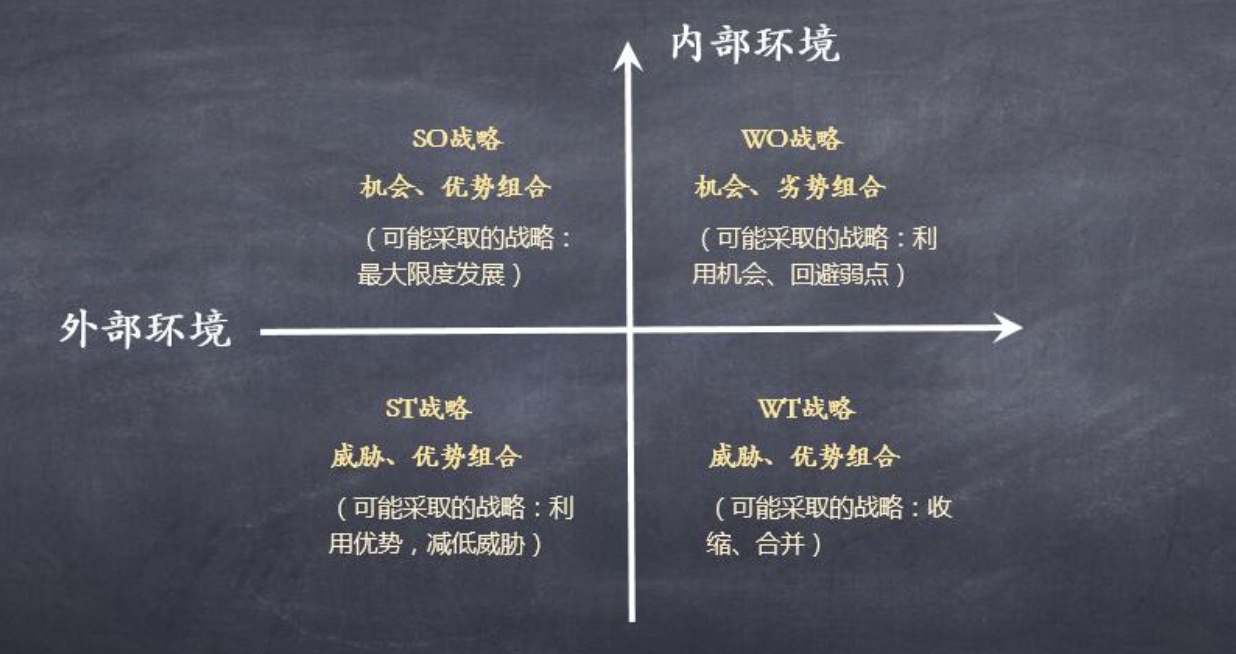
\includegraphics[width=1\textwidth]{fig/SWOT.png}
\end{figure}

\section{KOL}
关键意见领袖(Key Opinion Leader,简称KOL)是营销学上的概念,通常被定义为:拥有更多、更准确的产品信息,且为相关群体所接受或信任,并对该群体的购买行为有较大影响力的人。

在营销学上,为各厂家宣传的专家或权威被称为“关键意见领袖“,通常被定义为:拥有更多、更准确的产品信息,且为相关群体所接受或信任,并对该群体的购买行为有较大影响力的人。

与“意见领袖”不同的是,关键意见领袖通常是某行业或领域内的权威人士,在信息传播中,他们不依赖其自身活跃度,也容易被承认和识别出来。

\subsection{典型特征}
第一是持久介入特征:KOL对某类产品较之群体中的其他人有着更为长期和深入的介入,因此对产品更了解,有更广的信息来源、更多的知识和更丰富的经验。

第二是人际沟通特征:KOL较常人更合群和健谈,他们具有极强的社交能力和人际沟通技巧,且积极参加各类活动,善于交朋结友,喜欢高谈阔论,是群体的舆论中心和信息发布中心,对他人有强大的感染力。

第三是性格特征:KOL观念开放,接受新事物快,关心时尚、流行趋势的变化,愿意优先使用新产品,是营销学上新产品的早期使用者。

\section{湖畔大学曾鸣演讲:没有方向,所有努力都没有结果}
\url{https://mp.weixin.qq.com/s/exGrfnVVpQYYkRpL3it2VQ}
\subsection{前言}
从100年前,商学院创立以来,大家都在尽可能用科学的方法把规律性的东西总结出来,这是科学的方面;艺术这一块大家都很熟悉,很多企业家天马行空、特立独行,非常有创造力,这部分是学校没法教的。

另外一部分也是容易被大家忽略,战略当中的很多事情本身就是人做的事情,是经验的积累,只能言传身教,只能手把手地教,从这个角度来说是肯定能学会的,但是另一方面学起来的成本和代价是很高的,因为\textbf{它不是可以量化、可以说得明白的东西,更多的是一种经验的累积和传承}。

我原来上课的时候最怕别人问我:怎么制定战略?

这个问题没法简单回答。这些不是三言两语能讲清楚,而且不同情况下差别往往很大。我想跟大家分享——手艺的经验和体会,科学的大家看书都可以明白,艺术的我也讲不了,所以我跟大家交流一下手艺方面的心得。

\subsection{战略起什么作用?}
具体展开战略的讨论之前,想跟大家讲一下战略在企业当中起到什么作用。

\subsubsection{企业三基石——使命(Mission):Why us?}
Mission是大家熟悉的使命,我自己的体会是:\textbf{一个真正好的企业一定有超越金钱之上的追求,没有钱是万万不能的,但是钱绝对不是万能的,对于一个好的企业来说,要想招到真正的人才,要想做出一番事业的话,肯定要给大家自我成就感,一种超出小我的大追求}。

为什么要有使命感?

\textcolor{red}{本质上是解决组织存在的意义,Why us?}

什么叫组织?

\textcolor{red}{组织是一群人走到一起,完成任何单个人不能完成的任务。什么样的人为了什么样的目的走到一起,这是企业存在的“终极目标”。}

如果仅仅以钱作为存在的目的,用战略学的角度来说是没有差异化,因为钱是过于同质化的东西,没有差异化就没有办法吸引到更好、更不一般的人才。

所以,使命感是一个企业非常重要的基石。

\subsubsection{企业三基石——远见(Vision)}
Vision,很多人翻译为愿景,但愿景带着太多的个人意愿,我一般把它翻成远见,就是看未来的能力,对未来的预测、把握。

为什么Vision这个词特别好?因为“看”是一个动词,能不能看到未来?未来在你面前能不能活生生的浮现出来?

\textbf{战略最重要的两个要求:一个是前瞻性,一个是差异化。}

前瞻性从何而来?

\textcolor{red}{第一,站得高、看得远。}

前瞻性的源头在于你对未来与众不同的判断,你比别人能够更早、更快、更清晰地看到未来可能展现出来的状态。

你能看到未来,自然就比别人走得更好。就像我们现在看过去,如果知道会有金融危机,今天的世界肯定完全不一样,遗憾的是我们没有这样的远见,能够预见会出现金融危机。

\textcolor{red}{第二,它决定的是What do we do? }

这一群人在一起干什么事情?才能实现组织的使命?远见是解决做什么事情的问题。

\subsubsection{企业三基石——组织(Organization)}
\textbf{Mission解决的是人的问题,Vision解决的是事的问题},但是人和事怎么融在一起?怎么样的人才是合适的人?

在什么情况下做什么事情,其实这就是组织。组织解决“how do we do it”的问题。

我在这方面是门外汉,但是有一些简单的观点跟大家分析,比如:团队。我看了很多关于团队的讨论,我觉得都不在要害,\textcolor{red}{大家提倡团队精神,其实团队不是一个原因而是一个结果,是各方面的东西都对了以后出来的结果,团队是很难事先做出来的}。

所以,组织最重要的要求就是正确的人、正确的事、正确的方法——怎么有机融合在一起?

\textbf{把合适的人和事融合在一起的,就是执行力的核心。}

其实Who和What结合在一起就是大家非常熟悉的 “志同道合”,只有志同道合才有团队的可能性。

方向不一样,方法不一样,道不同不相为谋,没有志同道合的前提条件,就不可能成就一个好的团队。

很多企业一开始并没有使命和愿景怎么办?

像阿里巴巴这样在1999年成立的时候就有明确的愿景的企业是非常非常少数的。即使是这样,其实马云在1999年创立阿里巴巴之前也已经有过四年的创业经验,所以那个使命也是在这过去的经验当中提炼出来的。

有的人是因为有比较强的使命,所以才会愿意暂时放弃一些短期的利益,去更努力地看长期的发展趋势,因为这样才能真正把企业做的长久,实现自己的使命。

所以,使命感是企业愿意去思考远见的一个很常见的前提条件。

但反过来,\textcolor{red}{也有一些人相对来说是远见驱动的,他是因为看到了未来,在实现这个未来理想的过程中使命感越来越强}。

所以通常来说使命是在企业从小到大的过程中逐渐明确、逐渐强大起来的,它反过来也会对一个好企业的基因带来更大的促进作用。

这是我自己总结出来的基业常青企业的三个基石。

\textcolor{red}{能做好一个算是一个好企业;能做好两个大概是一个优秀的企业;能做好三个肯定是卓越的企业。}

\subsection{战略的思考}
什么是战略思考?

我觉得战略思考是一种可以培养的能力。对于企业来说,只要是进入管理层的人,都要慢慢培养战略思考的能力。

如果到了总监层面没有战略思考的能力,这个企业的执行力会大打折扣的,因为中层管理人员承上启下,没有战略思考的能力就没有办法接住上面往下传的想法,也很难把一线的很多情况进行提炼,有效地往上传递。

同时,在战略制定的过程中应该把中层融入进来。磨刀不误砍柴工。在战略制定上让他们多参与一些,其实大幅提升了执行的效率,因为他们理解了某一战略制定的逻辑和背景,而且有参与感,就能更积极主动地执行。

\subsubsection{前瞻与知止}
\textbf{战略思考当中最核心的是远见。}

\textcolor{red}{远见是战略判断的前提和假设,是战略前瞻性的基础}。从未来看现在的企业有战略,从现在顺着往前走的企业没战略。做事情前先想一下三年以后产业格局会怎么演化。

\textcolor{red}{“以终为始”才是战略思考}。如果说今天是这样,大家都这样,所以我也要这样,这是最典型的没有战略。一窝蜂而上,什么流行做什么,永远在跟风,永远赶下一个潮流,这是典型的机会导向。

判断一个企业有没有战略思考,最简单的就是看这个企业的人内部讨论的时候,会不会经常讲未来会怎么样,倒着推怎样才能推到这。

\textcolor{red}{成功人士的基本思考方法也是倒着推,因为方向都没有的情况下,所有的能量都是毫无意义的,能量和方向在一起才是作用力,战略更多的是告诉我们方向,给你一个方向感}。

有一个词叫“知止”,“知止”是李嘉诚先生挂在他办公室的条幅。“止”是终点的意思,因为你知道终点,所以才知道这个路该怎么走。

“知止”源自《大学》里的一句话:“知止而后有定,定而后能安,安而后能虑,虑而后能得”。

大部分的时候,“虑”可以理解为思考和计划,是所谓的战略规划,而“虑要有所得”,前面还有这么重要的三步。

我们经常讲企业家最难的是什么?

\textcolor{red}{“耐得住寂寞、挡得住诱惑”,而这两个的前提都是有定、有安,有这两个才能有虑,因为心安才能理得}。这是我讲的战略第一步,其实看得越清楚,才越不为外界所惑,越能够形成自己的判断。

我们讲\textcolor{red}{总裁的关键在裁,裁者决也,能做判断、能做决定,不管决定面临多大的不确定性,总要摁按钮}。这是战略思考的第一个核心,知止、产业终局判断、前瞻性,这是战略非常重要的第一步。

\subsubsection{取势与取实地}
当你知道战略的大致方向,你就知道起点和终点。下一步要决定的就是战略的路径选择。

你选择什么样的路径?

\textbf{直线走是不可能的,没有企业可以走直线}。我给大家讲个常见的思考方法:

大家经常会讨论,到底是“取势”还是“取实”?是落地为安还是能够构建一个大格局。战略很有意思的一点——你一直寻找动态平衡。

\textcolor{red}{战略到了最后就是动态的平衡,找的就是一个度}。所以,企业发展很重要的一点,“度”是一个动态平衡,“度”当中决定了企业发展的节奏。

当你快速膨胀之后,要有沉淀下来消化吸收的过程,要不然就像我们看到的一些企业圈地,满世界的圈,最后一个浪打回来一定像多米诺骨牌一样快速往回倒,连停的间隙都没有。

\textcolor{red}{所以,节奏和度是非常关键的,在取势和取实地中掌握动态平衡。这中间,根据不同的情况有不同的判断}。

\subsubsection{如何破局}
大家对未来有一个相对朦胧但是比较清楚的大方向的情况下,第一个切入点是最关键的。

我们之前讨论的时候,讲得最多的一句话就是:有了一张战略图之后,一定要找到一个地方是一刀捅进去就会流血的,闻到血腥味大家自然会冲上来,这张皮一定能被撕开,如果4、5个点都是拿小钉子敲,敲了3年下来没有一个点是敲破的,所有人都崩溃了。

重要的是一定要找到一个点切入,把它做深做透,彻底的把这个桩打进去,再去渗透,扩张。

\textcolor{red}{“眼高手低”,我是把它当作褒义词用的,立意一定要高,入手一定要低,这才是一个很好的战略结合。立意不高就没有格局,没有势成不了大器;入手不低你不可能有突破、有积累}。“手眼”配合,战略才能有效落地。

\subsection{战略=想做$\cap$可做$\cap$能做}
前面讲的是战略思考。接下来跟大家讲到底什么是战略? 战略的内容是什么?

\textbf{战略说白了非常简单,就是决定一个企业该做什么,不该做什么}。有所不为,才能有所为,大舍才能大得。舍得本来就是一个佛家的词,舍得,舍得,不舍不得。

\textcolor{red}{第一,你想做什么?你的目标、理想是什么?什么能让你兴奋? }

\textcolor{red}{第二,外面有什么机会,什么事是可做的? }

不同的时候的确有不同的机会。这就是我前面讲的远见,最核心的是判断什么是大机会,什么是小机会。对远见的讨论可以推导出哪些可做,哪些不可做,哪些可大做,哪些要小做。这是对外部机会的判断。

\textcolor{red}{第三,什么东西你能做?你有什么样的资源、人或者组织建设的能力?}

想做,可做,能做,这中间的小小交集,才是你真正该做的,这就是你的战略。

\textcolor{red}{想做——大家想一想,很多事情,如果不是那么想做,有点勉强的话,十有八九这个事情最后做不好}。因为这件事情本来就够难了,你的心里还有疙瘩,还做得不甘不愿,最后能做成的几率很少。

\textcolor{red}{可做——可不可做,是对机会成本的判断。大部分的企业做投资决策的时候进行了可行性报告,可行性报告计算的是这个项目本身的净现值够不够高,这是财务的分析}。战略分析的是为了追逐这个机会而放弃的另外的最大机会是什么。战略为什么难,是因为事后都没办法盖棺定论。事后你可能会觉得这件事情亏大了,抓住小兔子却放过了大山羊。对机会的判断就一定要想机会成本的概念。

\textcolor{red}{能做——能做就是一个企业的能力,能做也有两个动态的统一。能力的培养需要资源和时间投入}。说得极端一点,能力建设也就是人有多大胆就有多高产,组织能力没有天生的,组织能力是逐渐培养出来的。从这个意义上来讲,你可以根据战略目标培养人才,但反过来能力的培养是极耗资源和时间的,特别是时间。能力的培养是没有捷径的。所以从这个角度来说,企业并不能万能的。

\textbf{能力永远是相对的概念,自己做得好不好不算数,能不能比你最好的竞争对手做得好那才叫核心竞争力,才是差异化能力}。

大部分企业想的是能不能把这件事情做起来,挖两三个人组建小团队的确能把这件事情做起来,但是你很可能做得并不够好,更不可能当这个行业竞争越来越激烈、情况越来越残酷、利润越来越低的时候,有限的能力不可能抵挡这个市场整合时候的强大压力。所以,“能做”一定是一个相对概念。

\textcolor{red}{所以,一个人最重要的是发挥自己的长处,做到淋漓尽致,而不是拼命的补短板,因为补短板是永远补不够的}。

\subsection{战略演进的4个阶段}
每个人讲到战略时都有一套自己的思想,但我后来发现大家对战略的讨论容易引起争议,因为企业处在不同的发展阶段,主要矛盾不一样,战略也就完全不一样,战略本身的特征也有所区别。

\subsubsection{战略尝试期}
从0到1是创业公司必经的一条路,也是非常难过的一个坎。这个阶段的企业还处于战略尝试期,简单说就是企业在创新过程中还完全没找到“北”,但创始人知道战略很重要。

不过,这里面也分机会导向型创业者和愿景导向型创业者,两种完全不同的风格。

\textbf{机会导向型创业者比较贴近市场,很接地气,知道自己现在要什么,会抓住一、两年之内很好的机会切入},比较有长远思考的人甚至能抓住两、三个机会。这种创业者会意识到自己要形成战略思考能力,逐步的把企业往上拔。

\textbf{而愿景导向型创业者在刚开始创业的三、四年是极为痛苦的,因为他找不到切入点,更多的是在思考未来},但这个未来跟现实隔得太远,怎么投射到创业当下是比较难的,需要不断地试错。

很多企业会卡在这里,你尝试太多,机会窗口可能就没了,或者投资人不愿意陪你玩了。

所以,愿景导向型创业者在0到0.1的阶段是最难的,但从0.1到1会是最快的,因为他已经花了很长时间思考战略问题,只要产品一出来,他就知道怎么把它做大,后劲很足。

\textbf{总体来说,当企业处于战略尝试期时就是创新试错,思考如何让愿景逐渐变得越来越清晰,找到合适的切入点,这个时候创始人是唯一的驱动力,因为只有你才能hold住这样一个极为艰难的磨合过程}。

\subsubsection{战略成型期}
而战略成型期重要的是收敛,当创业者找到感觉后能不能把它变成一个套路、一个战略、一个模型,这个时候团队要形成共识,因为最早可能只有创始人自己觉得战略是对的,现在就需要让整个团队理解并认可它。

我\textbf{判断一个企业,特别是平台型企业有没有进入战略成型期,看的是企业营收能不能在两、三年内翻十倍,因为你找对了方向,企业就一定会有一个引爆阶段,这个增长是可以实现的}。

这是企业处于战略成型期非常典型的一个特点,只要切入点找得非常准,企业的发展就会有引爆点,然后你的资源积累在这时就会出现第一轮爆发,企业的整个势能会被带起来,团队也开始逐渐成型。

\subsubsection{战略扩张期}
第三个阶段是战略扩张期。这时,企业的战略要清晰,只有清晰的战略才能被分解,才能被不懂战略的人去局部执行。然后要讲究业务模式,并且这个模式能够分解下去,依靠下面的组织来执行,而不再是核心团队了。

创业者在战略扩张期要有组织能力,还要懂得找杠杆,搞清楚你到底要靠什么杠杆来实现企业的高速发展?是资本杠杆、组织杠杆还是业务杠杆?

\subsubsection{战略执行期}
最后一个阶段就是战略的高效执行期,所有套路都很熟了,剩下的就是速度问题。这个时候,企业要做的是优化运营模式,因为你已经找到了影响企业发展的两、三个关键点,这个关键点就类似零售里说的平米绩效。

此时,文化就要发挥作用了,因为整个团队单靠创始人已经管不过来了。关键的是,企业前期发展中积累的文化能不能自然地释放出来,或者说所谓的非正式文化元素能不能够降低组织的运营成本。

所以,大家可以思考一下自己的企业当前处于四个阶段中的哪一个阶段,这对创业者可能有正面的导向作用。

比如0.1到1就是企业引进人才最好的时候,因为原来的团队可能不太具备高速成长的能力,创业者需要引进一些年轻人跟着你快速成长,这些人会成为下个阶段企业组织的leader,那个时候你已经不可能直接带团队了。

当企业处于战略扩张期的后期时,创业者是能够往后退的,把更多事情交给团队来打理,但当企业在战略成型期时是万万不能往后撤的,因为很多东西还没成型,需要创业者去判断、把握。

\textcolor{red}{因此,了解企业所处的战略阶段,会帮助创业者找准自己的角色定位}。

\subsection{当战略决策成为常态}
\textbf{今天的战略早就不是一次决策,而是持续决策}。

因为我们面临的是一个高度不确定、存在巨大变化的时代。不确定性成了常态,以至于我们过去学习的很多战略也好、组织也罢的内容,都需要进行一定程度的扬弃。

这将导致我们思考方式彻底发生变化。我们很难强迫自己给出一个三年的准确判断,因为任何判断一定是错的,你只能作一个初步判断,然后根据反馈做迭代和优化,你只要比别人早一点接近未来就够了。但挑战在于,这套方法论是需要训练的。

\subsubsection{战略不再是CEO一个人的事}
从这个意义上看,\textcolor{red}{战略能力不再只集中于CEO,某种程度将成为高管团队的核心素养}。

因为企业需要经常作出重要决策,战略决定变成了这个组织的持续产出。而但凡是战略决定,一般也都事关生死,而环境的变化速度又那么快,这就倒逼企业必须强化自己的战略能力。

为什么以前会有麦肯锡这样的咨询公司?

是因为在原来的传统行业,企业作重大战略决策的周期往往是十年或二十年,所以不值得投入精力去培养战略能力,也没有办法培养出战略能力,因为作重大战略决策的机会很少。

所以大家都把能力外包给一个公司,他们的方法论磨得比较好,然后用这套方法论来帮助企业做长期的十年战略规划,即便需要花费数千万,但一想能管十年,也觉得值。

但今天,当你的组织需要持续不断地输出战略决定,战略就必须变成你的核心能力,同时它还要成为组织的内生能力。

\subsubsection{战略和执行不再割裂}
今天一线员工的决策都很可能产生战略影响。因为你很多时候输出的只是一个战略意图或者战略想象,当它们被传递到一线,尤其是遇到具体场景时,如何决策就成了一线员工的事情。

\textbf{本质上,一线员工的行动就是组织实际实施战略的一部分},而不像过去,员工仅仅作为执行者。战略跟执行不再割裂。

过去,战略决策都是自上而下,战略目标层层分解后,下面的员工用标准化的动作去完成,然后实现一个确定的KPI。\textbf{今天组织面临的挑战是,如何通过分布式协同的方式来完成战略实施?}

为什么今天都会抱怨公司内部协同太难?

\textcolor{red}{因为以前压根儿不需要协同,今天则完全相反,达成目标需要太多人的共同参与}。从这个意义上看,战略在第一天就被分解了下去,执行本身就蕴含着战略,它成为战略反馈的一部分。

但今天的这种分解在颗粒度层面和过去又有不同,它更像是一个有机演化的过程,需要的是共同创造。

为什么现在“共创”这个词也变得这么流行?因为战略越来越成为一个共同创造的过程,更多的人需要被卷入。这是一个需要创造力的时代。

福特当年有句名言,“我希望员工来的时候不要带脑袋,带手跟脚就行了”。但今天你一定希望所有的员工都把脑袋带来,但是你要管脑袋就得管心,心不在,脑袋就不在。

心怎么管?

你自然就要讲使命、愿景和价值观。这和过去是完全不同的一套逻辑和机制,因为你要的是他们的大脑,而不再是标准化的动作。

德鲁克讲过一句非常经典的话:\textcolor{red}{“没有人有能力预测未来,预测未来最好的办法就是创造它。”}这句话在今天看来尤为贴切。

\section{到底什么是商业模式?}
\url{https://mp.weixin.qq.com/s/OmaQd_TT4HtN7RB7zhZY3A}

这个世界上有很多公司,是靠商业模式赚钱的。比如Uber、滴滴,几乎不拥有出租车,却是市场上最大的出租车公司。比如airbnb,几乎不拥有任何一家酒店,却是全球最大的酒店出租方,比任何一家酒店连锁集团都大。再比如阿里巴巴,淘宝上卖的大部分商品都不属于阿里巴巴,但是不妨碍阿里巴巴成为全国最大的电商平台。

\textcolor{red}{这些公司连产品都没有,他们就靠纯粹的商业模式赚钱。}这就是商业模式的力量。

那么,到底什么是商业模式?理论界对这个话题做了很多研究,分了各种各样的门派。我把它总结为2,3,4,6,9,几个模型,今天,先通过这几个门派给你简单介绍下,到底什么是商业模式。

\subsection{2要素模型}
\begin{figure}[H]
    \centering
    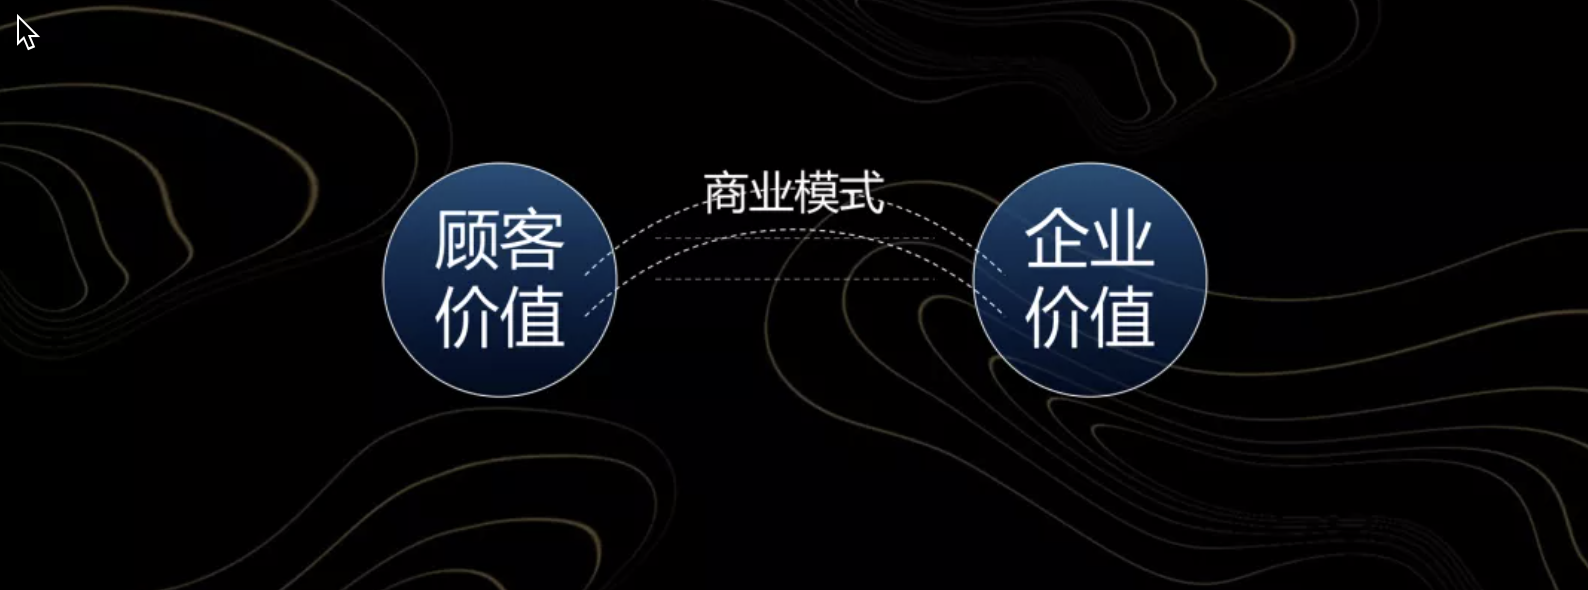
\includegraphics[width=1\textwidth]{fig/BusinessModel_1.png}
\end{figure}
什么叫2要素模型?\textcolor{red}{商业模式最基本的表述,就是我们一定要发明一种交易结构,这种交易结构首先一定是让顾客获得价值,然后同时我们企业也要获得价值。}

这样,这个商业模式就成立了。这是最朴素、最简单的商业模式。

\subsection{3要素模型}
\begin{figure}[H]
    \centering
    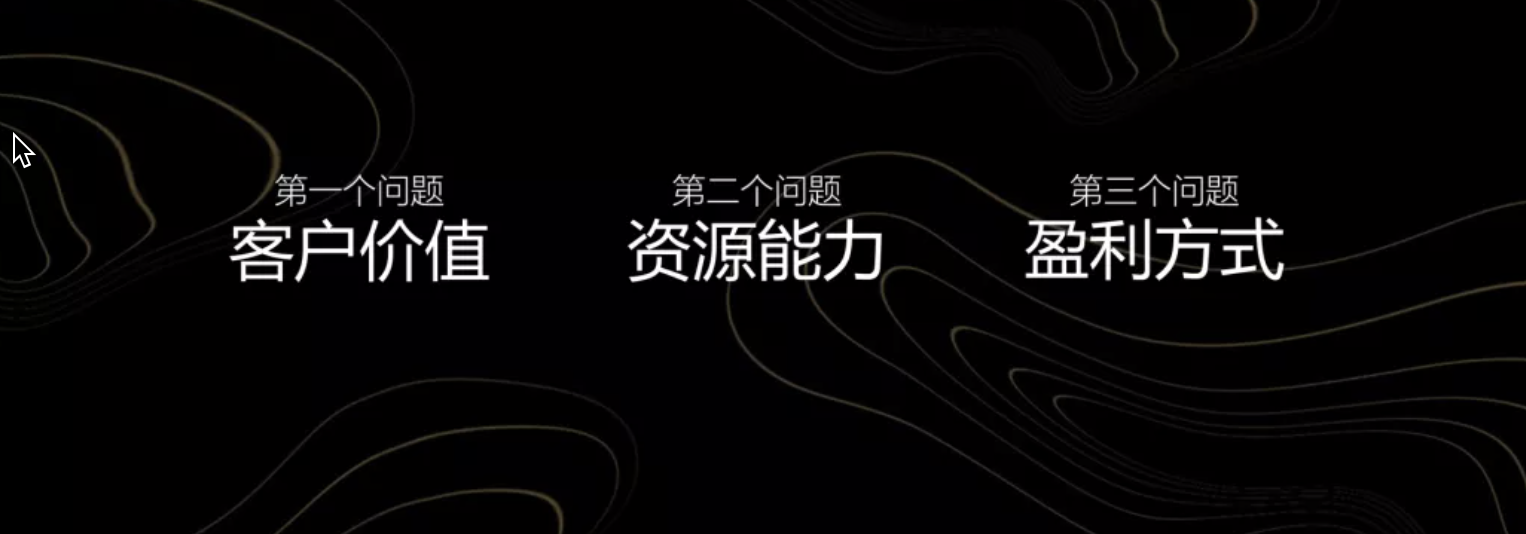
\includegraphics[width=1\textwidth]{fig/BusinessModel_2.png}
\end{figure}
3要素模型的意思是,\textcolor{red}{任何一个商业模式都要研究至少3个问题}。

\textcolor{red}{第一个问题,你为,什么人提供什么价值?}

可能会有同学认为这个问题有点虚。说,我为客户做的一切都是有价值的。或者有的以客户为中心的企业会说,客户需要的,就是我们提供的,我们要为客户提供一切他需要的价值。其实,这些都不是你确定给客户提供的价值。那什么才是?比如,你开了个瑜伽馆,你给客户提供练习瑜伽服务。这是你提供的价值。

\textcolor{red}{第二个问题,凭什么是你?}

你的瑜伽馆生意还不错。可为什么是你开得不错呢,别人不行吗?你的瑜伽馆生意还不错。是因为,你恰好找到了一个很多人想练瑜伽、潜在客户特别多的地方吗?还是因为你的瑜伽教练非常专业?还是因为你有独特高效的运营方法?总之,你一定有一种独特的资源能力,才能把你的瑜伽馆开得还不错。这个能力,只有自己能回答。

\textcolor{red}{第三个问题,你的钱是哪来的。}

或者说,你的利润从哪里来?如果前面两个问题回答好,这个反而最好回答。因为你独特的能力,喜欢瑜伽的人爱来你这里练习,自然会付钱给你。水到渠成。

所以,要想赚钱,你必须要回答前面两个问题,然后你才有机会回答这第三个问题。

很多人默认商业模式就是盈利模式。但是你看到这个模型之后,你要明白,\textbf{盈利模式只是商业模式里面的一部分}。最重要的反而是前面两个问题。最重要的反而是前面两个问题。

\subsection{4要素模型}
\begin{figure}[H]
    \centering
    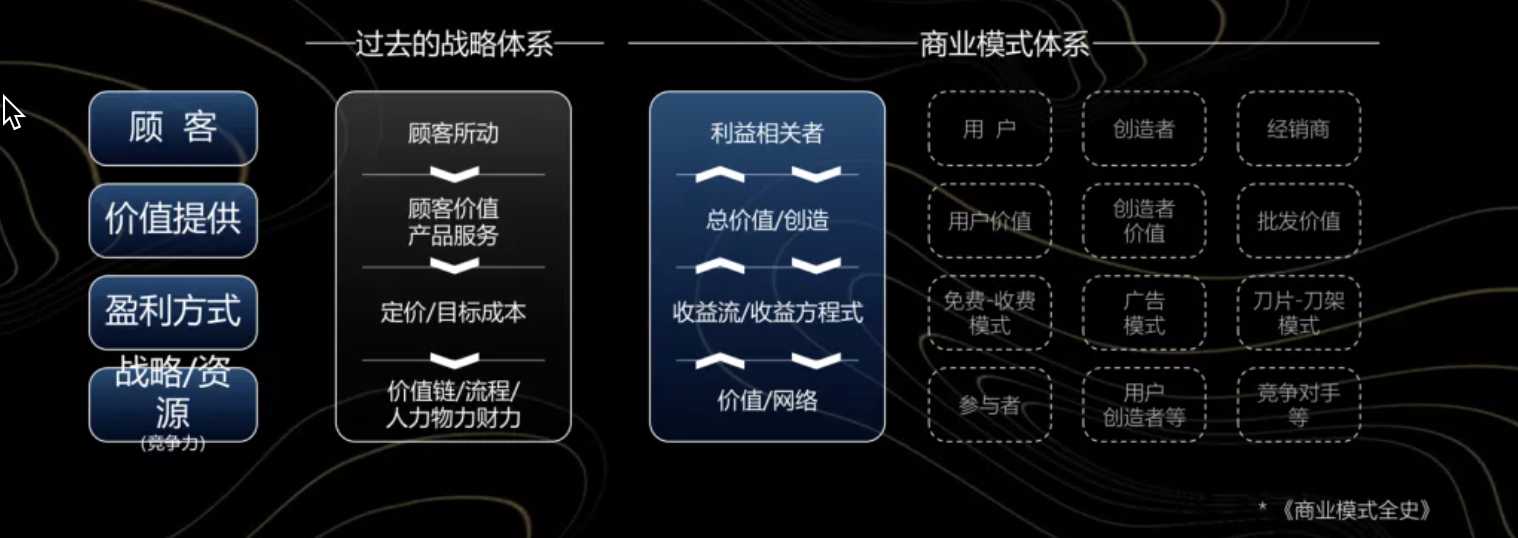
\includegraphics[width=1\textwidth]{fig/BusinessModel_3.png}
\end{figure}
什么是4要素模型? 这是日本早稻田大学商务学院客座教授三谷宏治,在他的著作《商业模式全史》中提出的一个模型。 4要素模型和刚才提到的3要素模型没有特别大的区别。 它的4要素分别是什么呢? 它的4要素分别是什么呢? 

\begin{itemize}
\setlength{\itemsep}{0pt}
\setlength{\parsep}{0pt}
\setlength{\parskip}{0pt}
    \item 你的客户是谁? 
    \item 你给客户提供什么价值? 
    \item 你是怎么盈利的?  
    \item 你的核心竞争力是什么? 
\end{itemize}

\textcolor{red}{对应的4个要素就是,顾客、价值提供、盈利方式、战略/资源。 }

是不是和3要素模型基本一样,只是把3要素模型里的客户价值(你为什么人提供什么价值)分别拆成了客户(顾客)和价值(价值提供)。 

但是4要素模型,真正的价值,不是把3要素模型拆成了4要素模型,而是\textcolor{red}{他提出了一个总价值创造的概念}。

什么叫总价值创造? 就是,你不应该只关注你的客户。\textcolor{red}{你还应该关注你的供应商、你的渠道、你的门店,你必须让所有的这些利益相关者,加在一起都能获得价值,才能叫总价值创造}。 

举个例子。 过去,从100斤花生,能榨25斤油。 你说,我厉害了,我改进了压榨工艺,在品质不变的前提下,我能榨出40斤。 别人的25斤,和你的40斤之间,那15斤多出来的油,是你多创造出来的价值。 那如何让合作伙伴、消费者也获得价值? 

\textcolor{red}{你可以把这多出来的15斤油,拿出5斤油分给消费者。 }换句话说,用户用同样的价格,可以买到30(25+5)斤油了。 他们会非常高兴地,从竞争对手那里,投奔你的怀抱。 然后,\textcolor{red}{你把另外5斤分给合作伙伴}。合作伙伴也非常高兴。 这样就有更多人愿意帮你卖油了。 还有5斤呢?留给自己。这是你应得的部分。 你说,这不是总价值创造啊,这是把我创造的价值(15斤油)分给了消费者(5斤)和合作伙伴(5斤)而已。 不是。\textcolor{red}{因为更多的消费者来找你买,合作伙伴销售的就越多,你赚得也就越多}。 

这时,如果你原来每年卖3吨油,现在就有可能卖30吨,300吨。 这种商业模式才做到了总价值创造,或者你也可以说这叫全局性增量。 这就是4要素模型。

\subsection{6要素模型}
\begin{figure}[H]
    \centering
    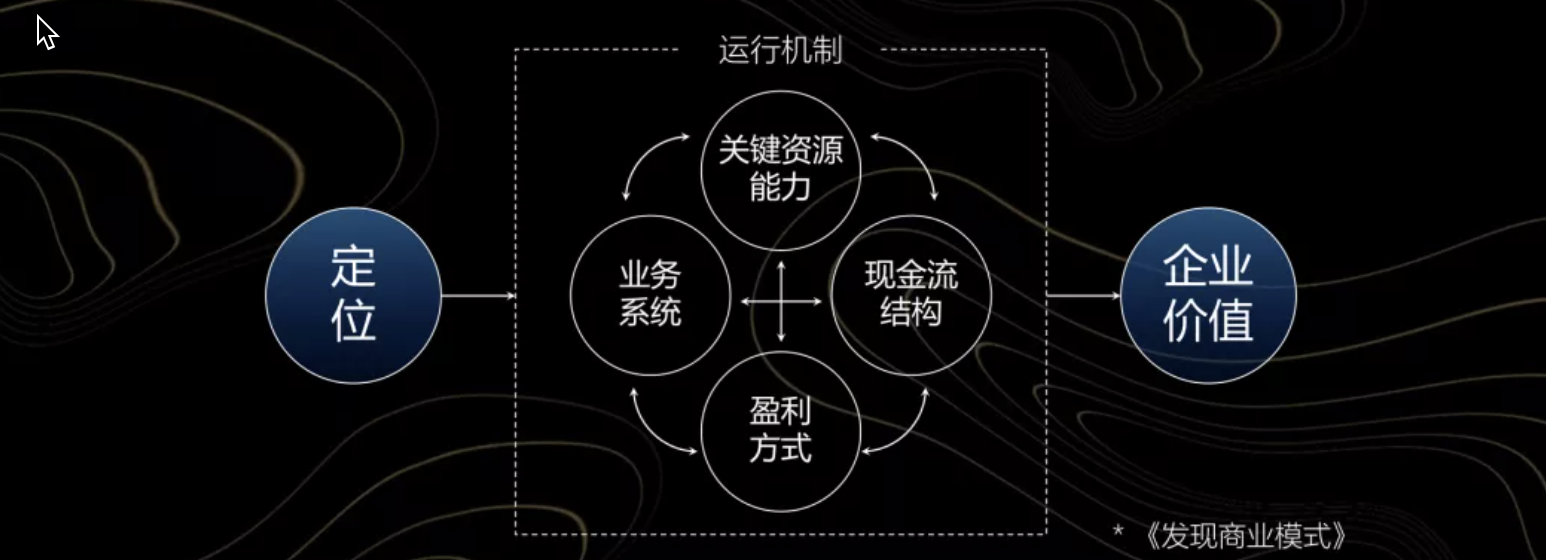
\includegraphics[width=1\textwidth]{fig/BusinessModel_4.png}
\end{figure}
6要素模型是魏炜教授提出的一个模型。他说,什么是商业模式?\textcolor{red}{商业模式就是利益相关者的交易结构}。

6要素模型第一要素是什么?

\textcolor{red}{定位}。什么是定位?你为什么客户提供什么价值,这就是定位。\textcolor{red}{有了定位之后,你就必须要搭建一个业务系统去做这个事。在搭建系统过程中利用你的关键资源、你的核心竞争力;然后梳理出你的现金流结构,完成你的盈利模式;最终实现企业价值}。这就是魏炜教授提出的6要素模型。在这里我就简单介绍下这个模型,不做延展,感兴趣的同学也可以找魏炜教授的书《发现商业模式》了解详情。

\subsection{9要素模型}
\begin{figure}[H]
    \centering
    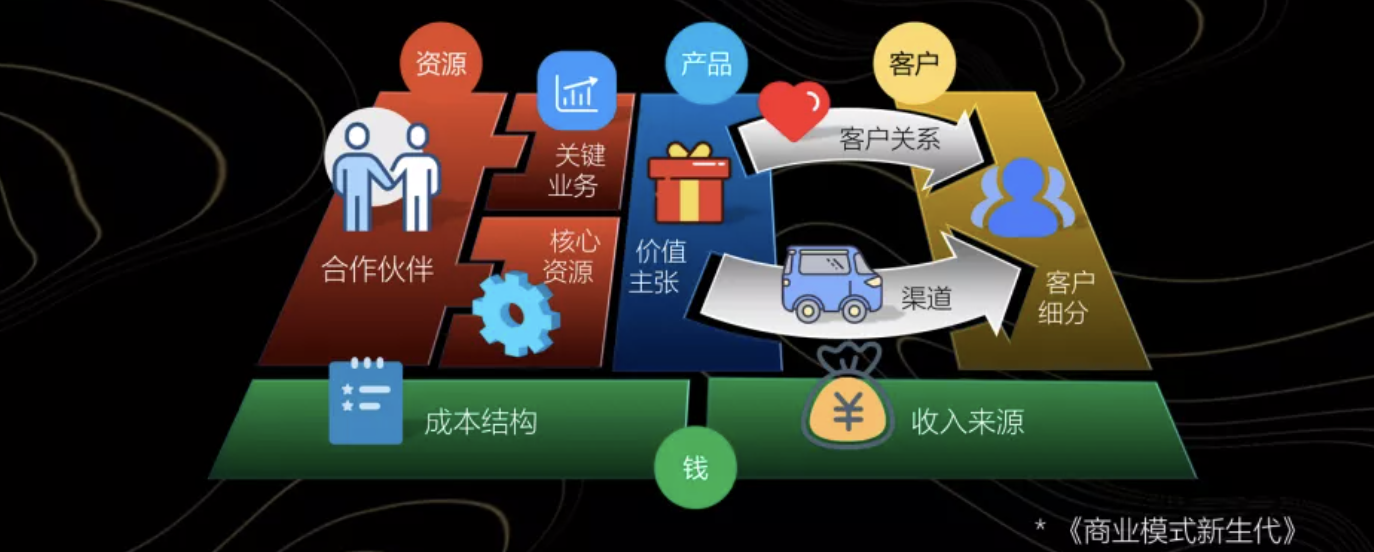
\includegraphics[width=1\textwidth]{fig/BusinessModel_5.png}
\end{figure}

9要素模型是亚历山大·奥斯特瓦德、伊夫·皮尼厄在他们的书《商业模式新生代》提出的模型。 什么是9要素模型? 简单来说,就是回答9个问题。 
\begin{itemize}
\setlength{\itemsep}{0pt}
\setlength{\parsep}{0pt}
\setlength{\parskip}{0pt}
    \item 第一,你的客户是谁?是如何细分的?(客户细分) 
    \item 第二,你和客户关系是怎么样的?(客户关系)  
    \item 第三,你通过什么渠道能找到这些客户?(渠道)   
    \item 第四,你为这些客户提供什么价值?(价值主张) 
    \item 第五,你通过什么关键业务给客户提供价值?(关键业务) 
    \item 第六,你的核心资源是什么?专利?人才?土地?(核心资源)   
    \item 第七,你的合作伙伴都有谁?(合作伙伴)    
    \item 第八,你的收入来源是什么?(收入来源) 
    \item 第九,你的成本结构是什么?(成本结构)  
\end{itemize}

前4个问题,其实就是3要素模型里的客户价值; 第5、第6、第7这3个问题其实就是3要素模型里资源能力; 而最后2个问题,就是3要素模型里的盈利方式。 这就是9要素模型。

 \subsection{最后的话}
 以上,就是商业模式里的2,3,4,6,9要素模型。虽然要素从2个变成3个、变成4个、变成6个,最后变成9个。看起来越来越复杂,但其实只是越来越精细。

回到最开始的问题,到底什么是商业模式?其实,所谓的商业模式,就是利益相关者的交易结构。作为企业家,如果对照你的企业,你也想做商业模式创新。那么我建议你,\textcolor{red}{你的商业模式一定要可以做到总价值创造,创造全局性增量}。一切的商业模式,都必须有全局性增量。如果没有,那所谓的商业模式,就是把你口袋的钱换到我口袋。

最后,我特别建议你问自己2个问题:1、我为什么人提供什么价值?2、凭什么是我?

回答完这2个问题,我期待那第3个问题“你的钱从哪里来?”的答案,会非常自然,水到渠成。期待。

\section{创新}
推荐阅读《创新者的窘境》《好战略,坏战略》

\subsection{克氏曲线}
\begin{figure}[H]
    \centering
    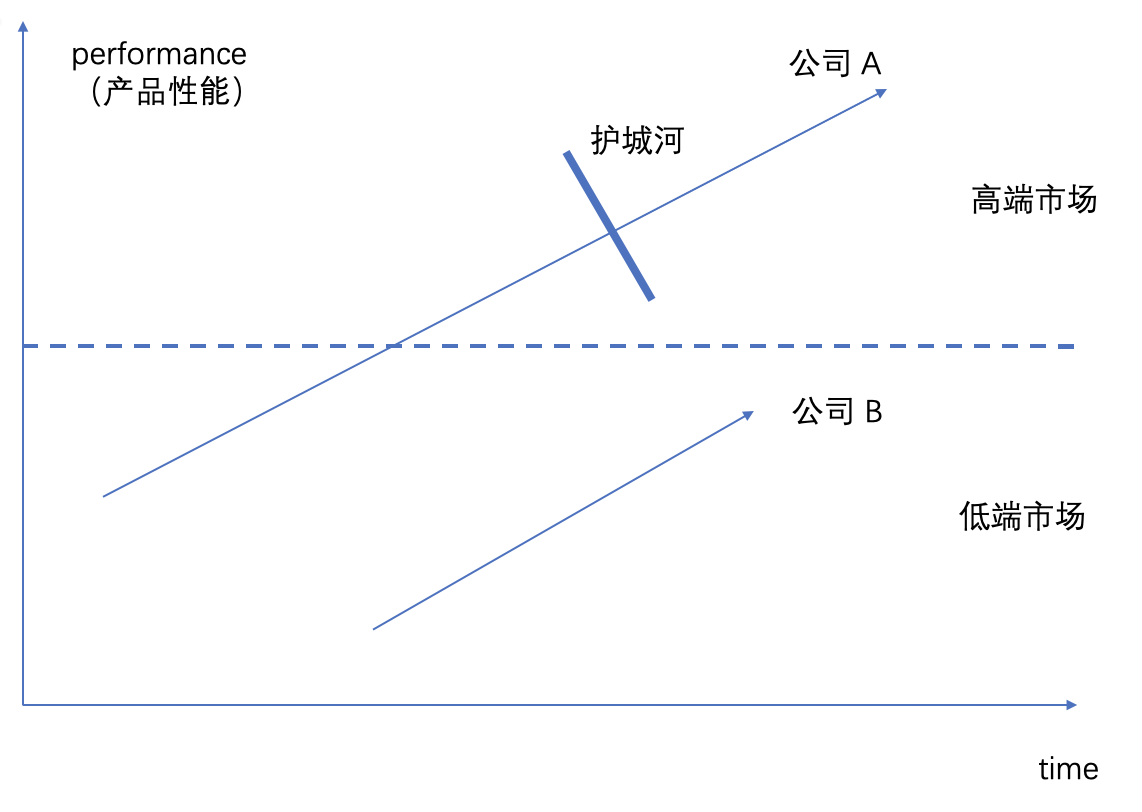
\includegraphics[width=.6\textwidth]{fig/Ke_Curve.png}
\end{figure}

企业进入右上角(高端市场)后,因为享受了高利润,所以只会倾向于做连续型创新,而不是颠覆型创新;入场的新玩家可以用简单的新性能,快速占领市场,这样原企业的护城河无法防住新玩家。

图上给出的是从低端进行颠覆,还可以采取 tesla 这种模型,进行高端颠覆;还有一种颠覆是跨界颠覆,类似于降维打击,在一个新平面上原平面的市场形成打击。比如柯达公司,在胶片时代就对数码技术进行了布局,但是结果却是被手机跨界颠覆掉了。

\subsection{复盘方式}
\begin{itemize}
\setlength{\itemsep}{0pt}
\setlength{\parsep}{0pt}
\setlength{\parskip}{0pt}
    \item 测试过却没成功的项目;
    \item 从竞争对手角度思考对方会怎么做;
    \item 有没有侧面战场;
\end{itemize}

\subsection{寻找第二曲线}
寻找下一个流量入口,并投资或提前布局;

思考企业增长过程中,能形成复利的资产是什么,比如数据,是持续积累的,可以持续发挥价值。

\subsection{四大增长引擎}
\begin{itemize}
\setlength{\itemsep}{0pt}
\setlength{\parsep}{0pt}
\setlength{\parskip}{0pt}
    \item 结构型增长-战略:PEST 模型/SWOT 模型;第二曲线与颠覆式创新;增长机会矩阵;
    \item 能力型增长-人才:创新型人才与组织创新;
    \item 生态型增长-资本:CVC 模型;分形与产业生态化;
    \item 效率型增长-技术:技术成熟度;
\end{itemize}

增长的类型:
\begin{itemize}
\setlength{\itemsep}{0pt}
\setlength{\parsep}{0pt}
\setlength{\parskip}{0pt}
    \item 肥肉型增长;
    \item 肿瘤型增长;
    \item 肌肉型增长;
\end{itemize}

高质量增长的特点:
\begin{itemize}
\setlength{\itemsep}{0pt}
\setlength{\parsep}{0pt}
\setlength{\parskip}{0pt}
    \item 可持续性;
    \item 盈利性;
    \item 投入产出比;
\end{itemize}

\subsection{宏观环境分析:PEST 模型}
\begin{itemize}
\setlength{\itemsep}{0pt}
\setlength{\parsep}{0pt}
\setlength{\parskip}{0pt}
    \item P-Political:国家或地区的政治制度、体制、方针政策、法律法规等;
    \item E-Economic:经济政策及经济发展水平;居民可支配收入、消费结构等;
    \item S-Sociological:人口结构、居民受教育程度、文化水平、价值观、宗教信仰等;
    \item T-Technological:技术的发展趋势及商业化速度,国家的重点投入和支持等;
\end{itemize}

\subsection{SWOT 分析模型}
横轴:优势(S),劣势(W);纵轴:机会(O),威胁(T)

战略类型:
\begin{itemize}
\setlength{\itemsep}{0pt}
\setlength{\parsep}{0pt}
\setlength{\parskip}{0pt}
    \item SO 战略-进攻战略;目标是充分利用外部机会、发挥内部优势;理想战略状况是内外部相互促进;战术运用上可以加速发展扩大优势;
    \item WO 战略:适用条件是存在有利的市场机会,但企业劣势可能形成阻碍,关键在于如何消除劣势带来的负面影响;从内部看,战略目标是通过机会来弥补劣势;
    \item ST 战略:理性博弈,利用内部优势减轻外部威胁;当面临某种威胁时,应考虑变革或收割;可适当撤回;
    \item WT 战略-防守战略:防御为主,减少劣势,回避威胁;如果面对的是市场威胁,建议寻求其他机会,或通过变革化解困境;
\end{itemize}


%\printbibliography
\bibliography{../ref}
\bibliographystyle{IEEEtran}
\end{document}
